\documentclass[11pt,a4paper]{article}
\usepackage[utf8]{inputenc}
\usepackage[spanish]{babel}
\usepackage[margin=2.5cm]{geometry}
\usepackage{graphicx}
\usepackage{booktabs}
\usepackage{hyperref}
\usepackage{amsmath}
\usepackage{float}

\title{Análisis Exploratorio de Datos -- Data Wrangling \\
\large Dataset Hubway: sistema de bicicletas compartidas de Boston (2011--2013)}
\author{Diego Raúl Rivas Huanca \\
Universidad Nacional de San Agustín de Arequipa \\
Maestría en Ciencia de la Computación -- Curso: Ciencia de Datos \& Big Data \\
Docente: Ana María Cuadros Valdivia}
\date{\today}

\begin{document}
\maketitle

\section*{Paso 0: Metadata}

Hubway fue el sistema público de bicicletas compartidas de Boston (hoy integrado a \textit{Blue Bikes}),
operativo desde julio de 2011. El dataset corresponde a la primera ventana de operación del sistema
(2011--2013).

El dataset se compone de dos tablas relacionadas:
\begin{itemize}
  \item \texttt{hubway\_stations.csv}: catálogo de estaciones físicas (dimensión, 142 registros).
  \item \texttt{hubway\_trips.csv}: bitácora de viajes individuales (hechos, $\approx$1.58 millones de registros),
  relacionada con \texttt{stations} mediante \texttt{strt\_statn}/\texttt{end\_statn} $\rightarrow$ \texttt{stations.id}.
\end{itemize}

Un registro de \texttt{stations} representa una estación de anclaje en un momento dado. Un registro de
\texttt{trips} representa un viaje individual cerrado (retiro de una bicicleta y su devolución).

\section*{Paso 1: Análisis del comportamiento de los datos}

\subsection*{Volumen}
\texttt{stations} tiene 142 registros; no requiere ningún tratamiento especial de escalabilidad.
\texttt{trips} tiene $\approx$1.58 millones de registros ($\approx$700 MB en memoria como \texttt{DataFrame}
sin optimizar de tipos). No es Big Data en sentido estricto, pero cálculos repetidos ya se sienten notoriamente
más lentos que con un dataset pequeño.

\subsection*{Duplicados}
No hay filas completamente duplicadas en ninguna tabla, y las llaves primarias (\texttt{stations.id},
\texttt{trips.seq\_id}, \texttt{trips.hubway\_id}) son únicas. Sí existe una duplicidad parcial con significado:
22 estaciones comparten el mismo código \texttt{terminal} en pares (una \texttt{Removed} y otra
\texttt{Existing}), lo que refleja reubicaciones/reemplazos de estaciones, no un error de carga.

\subsection*{Tipos de datos, discretos vs. continuos, rangos}

\begin{table}[H]
\centering
\caption{Resumen de tipos y naturaleza de las columnas de \texttt{trips}}
\begin{tabular}{lll}
\toprule
Columna & Naturaleza & Observación \\
\midrule
\texttt{duration} & continua (segundos) & rango [-6900, 11\,994\,460] -- valores imposibles presentes \\
\texttt{start\_date}/\texttt{end\_date} & temporal & texto, requiere \texttt{pd.to\_datetime} \\
\texttt{strt\_statn}/\texttt{end\_statn} & discreta (FK) & \texttt{float64} solo por presencia de nulos \\
\texttt{birth\_date} & discreta (año) & granularidad distinta a las fechas de viaje \\
\texttt{subsc\_type} & categórica binaria & Registered / Casual \\
\texttt{gender} & categórica binaria & Male / Female, con nulos \\
\texttt{zip\_code} & categórica & comilla inicial y longitud variable (artefacto de formato) \\
\bottomrule
\end{tabular}
\end{table}

Variables categóricas que requerirían codificación numérica para modelado: \texttt{subsc\_type},
\texttt{gender}, \texttt{municipal}, \texttt{status}.

\subsection*{Valores nulos}

\texttt{stations} no tiene nulos. En \texttt{trips}, \texttt{birth\_date} (77.8\,\%) y \texttt{gender}
(29.9\,\%) concentran la mayoría de los nulos. Al cruzar con \texttt{subsc\_type} se observa que el
100\,\% de los usuarios \textit{Casual} no tiene esos datos: es un patrón \emph{missing by design}, no
aleatorio -- el sistema no solicita esa información a quien compra un pase de un solo día. Adicionalmente,
entre los usuarios \textit{Registered} el porcentaje de nulos en \texttt{birth\_date} pasa de 1.1\,\% (2011)
a 100\,\% (2013), lo que evidencia un cambio de política de captura de datos, no un problema aleatorio de
calidad.

\subsection*{Distribución y medidas de tendencia central}

La duración del viaje está lejos de una distribución simétrica: media aritmética $\approx$1200\,s frente a
una mediana de 660\,s. La media geométrica ($\approx$678\,s) y armónica ($\approx$452\,s) están mucho más
cerca de la mediana, confirmando que unos pocos viajes extremadamente largos distorsionan la media
aritmética. La edad de los usuarios (17--79 años, disponible solo para un subconjunto) se ve razonablemente
simétrica.

\subsection*{Correlación}

No hay correlaciones lineales fuertes entre \texttt{duration}, \texttt{age} y las estaciones de
origen/destino; la única correlación moderada (r $\approx$ 0.34) es entre \texttt{strt\_statn} y
\texttt{end\_statn}, explicable por la numeración geográfica de las estaciones, no por una relación causal.

\begin{figure}[H]
\centering
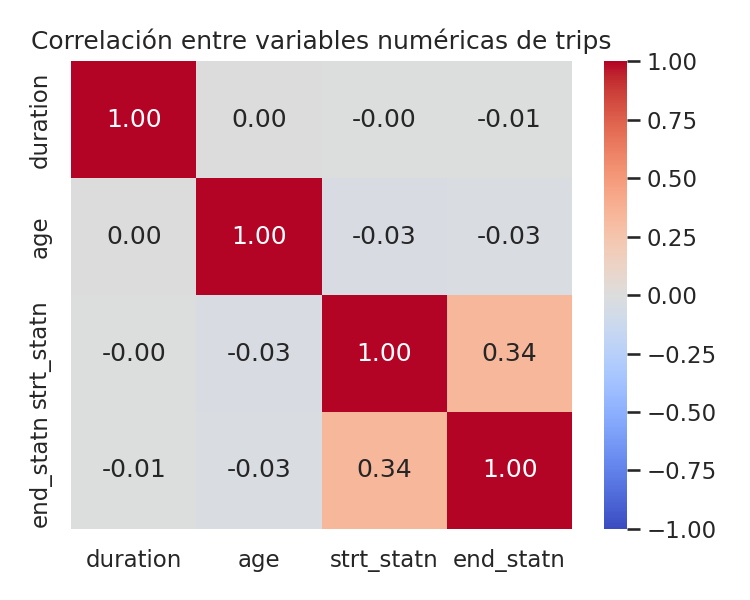
\includegraphics[width=0.6\textwidth]{figures/fig05_correlacion_heatmap.png}
\caption{Matriz de correlación entre variables numéricas de \texttt{trips}.}
\end{figure}

\section*{Paso 2: Análisis de outliers}

Usando el criterio de rango intercuartílico sobre \texttt{duration} (Q1=412\,s, Q3=1082\,s), el límite
superior de valores no atípicos es 2087\,s ($\approx$35\,min); un 6.6\,\% de los viajes lo supera.

Se identifican dos grupos de outliers con causas distintas:
\begin{enumerate}
  \item \textbf{Duraciones negativas (49 filas) y de 0 segundos (4389 filas):} físicamente imposibles --
  errores de sensor/reloj de estación. Se eliminan sin reparo.
  \item \textbf{Duraciones extremadamente largas (algunas de varios días):} eventos reales del negocio
  (bicicleta perdida, robada, o cierre automático del viaje por timeout del sistema al no registrarse
  devolución). No son errores de carga y se conservan para análisis operativo, pero se excluyen de
  cualquier estadística sobre ``duración típica de viaje''.
\end{enumerate}

\section*{Paso 3: Visualización}

\begin{figure}[H]
\centering
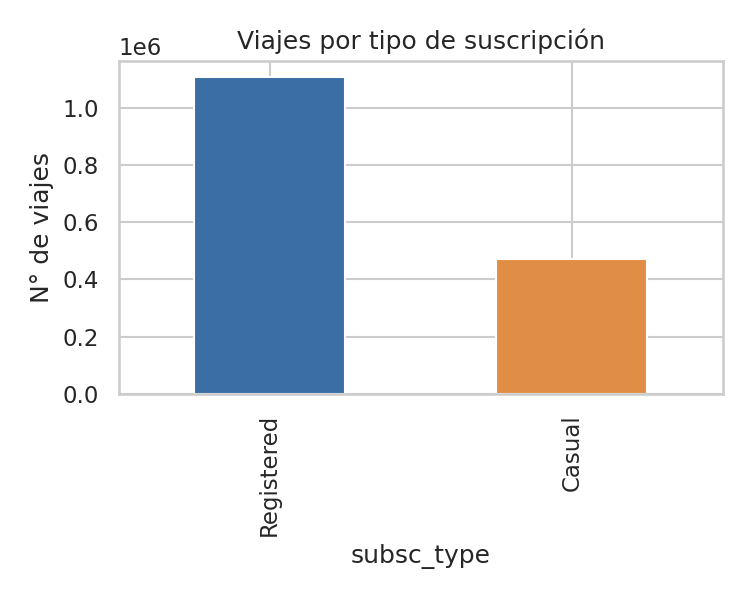
\includegraphics[width=0.48\textwidth]{figures/fig01_barras_subsc_type.png}
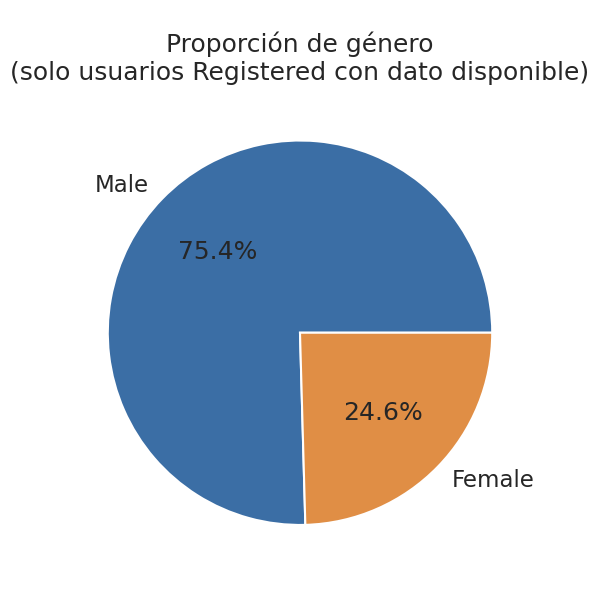
\includegraphics[width=0.48\textwidth]{figures/fig02_circular_genero.png}
\caption{Izquierda: viajes por tipo de suscripción (variable categórica, gráfico de barras). Derecha:
proporción de género entre quienes lo reportan (variable categórica, gráfico circular).}
\end{figure}

\begin{figure}[H]
\centering
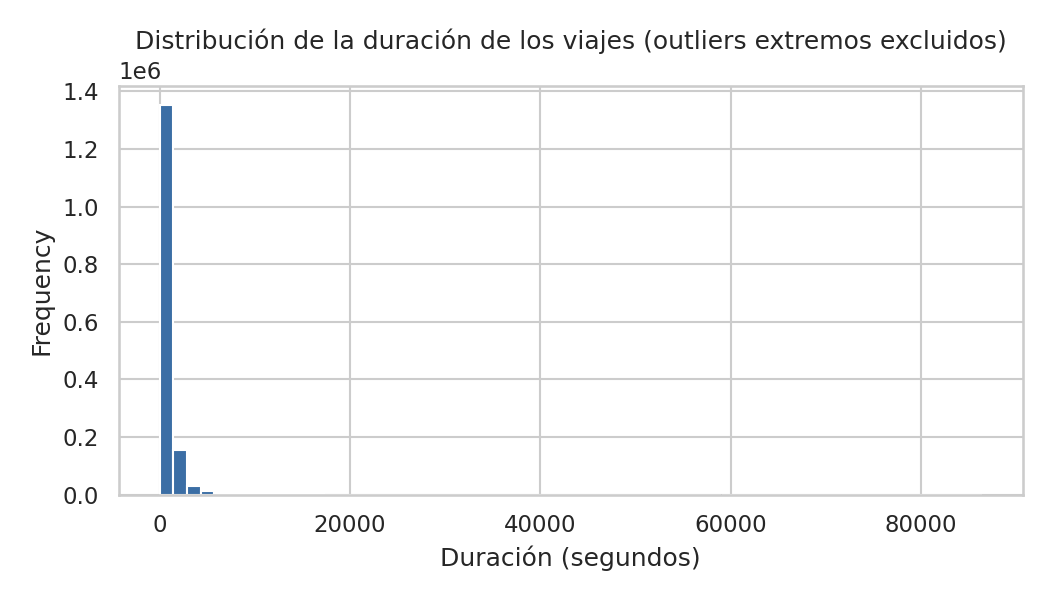
\includegraphics[width=0.48\textwidth]{figures/fig03_histograma_duracion.png}
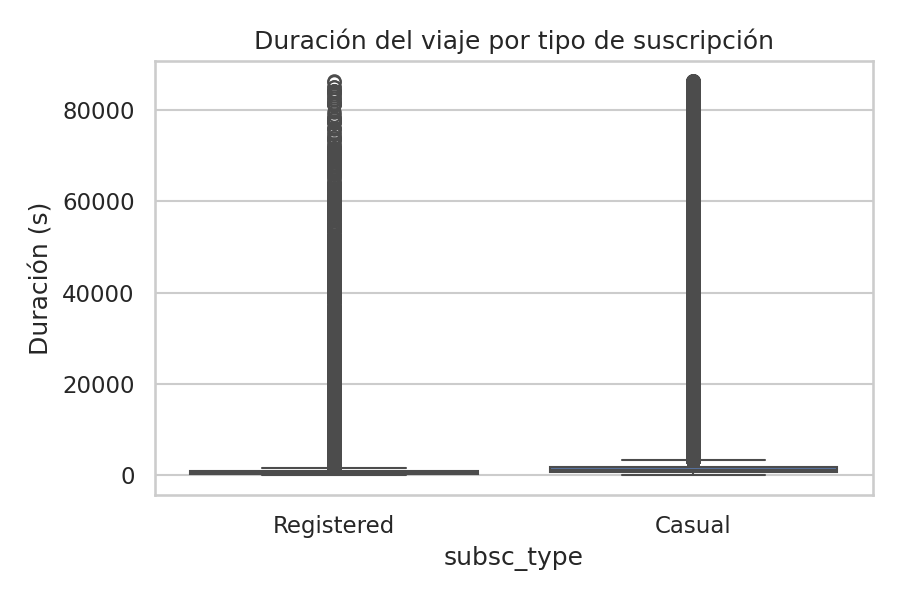
\includegraphics[width=0.48\textwidth]{figures/fig04_boxplot_duracion_subsc.png}
\caption{Izquierda: histograma de duración del viaje (outliers extremos excluidos). Derecha: boxplot de
duración por tipo de suscripción.}
\end{figure}

\begin{figure}[H]
\centering
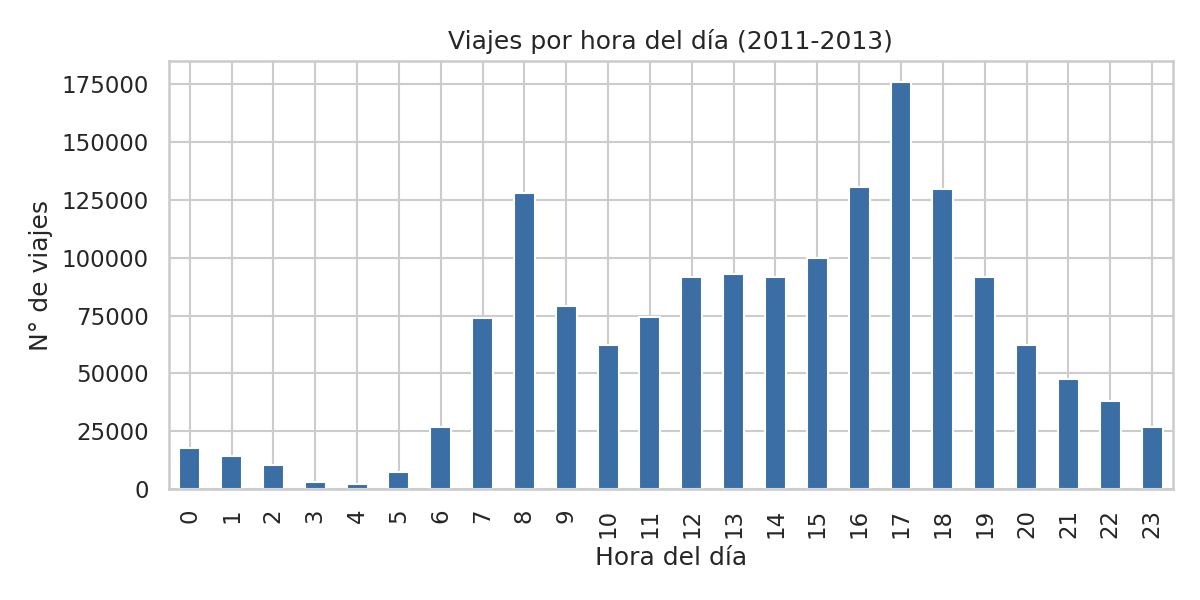
\includegraphics[width=0.48\textwidth]{figures/fig06_viajes_por_hora.png}
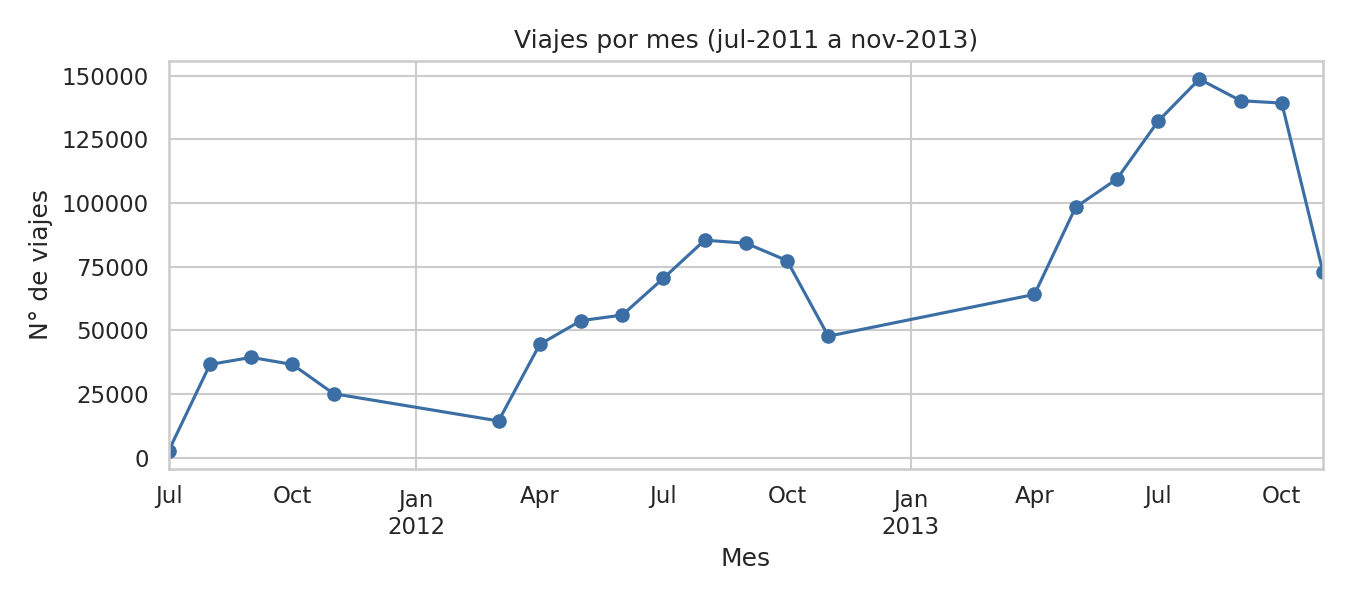
\includegraphics[width=0.48\textwidth]{figures/fig07_viajes_por_mes.png}
\caption{Izquierda: viajes por hora del día -- dos picos de \textit{commute} (8\,am y 17--18\,h). Derecha:
viajes por mes -- fuerte estacionalidad, el servicio se detiene en invierno.}
\end{figure}

\begin{figure}[H]
\centering
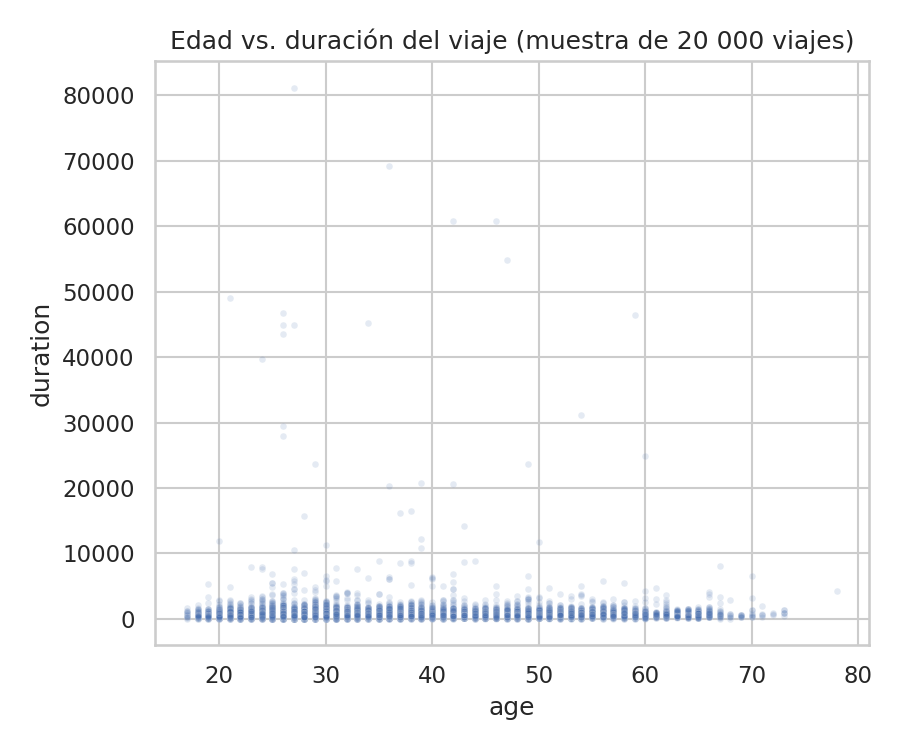
\includegraphics[width=0.55\textwidth]{figures/fig08_scatter_edad_duracion.png}
\caption{Scatterplot edad vs. duración del viaje (muestra de 20\,000 viajes).}
\end{figure}

El uso del sistema es predominantemente utilitario (patrón de dos picos de commute) y estacional (nulo en
los meses de invierno boreal), más que recreativo.

\section*{Paso 4: Problema potencial en los datos}

\textbf{Pregunta tiempo-espacio (dataset externo sugerido):} ¿el clima diario (temperatura, lluvia, nieve)
explica las variaciones día a día en el uso, más allá de la estacionalidad agregada por mes? Requeriría
cruzar \texttt{trips} agregado por día con un dataset externo de clima histórico de Boston (p. ej. NOAA /
Open-Meteo), uniendo por fecha.

\textbf{Como problema supervisado (predecir \texttt{subsc\_type}):}
\begin{itemize}
  \item Columna de salida binaria: Registered (70\,\%) / Casual (30\,\%) -- desbalance moderado, no extremo.
  \item Features candidatas: hora del día, día de la semana, duración, estación de origen/destino, mes.
  \item \textbf{No usar} \texttt{birth\_date}/\texttt{gender} como features: son nulas en el 100\,\% de los
  Casual por diseño, por lo que su uso constituiría \textit{data leakage}.
  \item Problema dependiente del tiempo: la composición de usuarios cambia con la estación del año.
\end{itemize}

\section*{Conclusión}

El dataset Hubway es de tamaño moderado, con una tabla de estaciones limpia y una de viajes con problemas
de calidad reales y bien identificables: outliers de duración con dos causas distintas, y un patrón de
nulos estructural (no aleatorio) ligado tanto al tipo de usuario como a un cambio de política de captura de
datos en 2013. El uso del sistema es claramente utilitario y estacional. Estos hallazgos deben guiar
cualquier modelado posterior: qué variables son seguras de usar como \textit{feature}, cuáles filtrarían la
respuesta, y qué subconjunto de datos usar según la pregunta.

\end{document}
